\documentclass[12pt]{article}
\usepackage[margin=0.5in]{geometry}
\usepackage{graphicx} 

\title{Autocorrelation in Weather: Are temperatures of one year significantly correlated with the next year (successive years), across years in a given location?}

\author{Amy Solman \\
MRes. Computational Methods in Ecology and Evolution - 2019\\
Imperial College London\\
Biological Computing in R}
\date{October 2019}

\begin{document}
	\maketitle

\section{Introduction}
Lag one-year autocorrelations of temperature are a well documented phenomena, particularly in North America \cite{madden1977estimates}. Understanding of temperature autocorrelation is an important tool in predicting future temperatures with respect to climate change \cite{mearns1984extreme}. This report examines mean temperature data taken from Key West, Florida, US, between 1901 and 2000. We aim to assess whether temperatures of one year significantly correlate with the next year (successive year), across years at our given location. Using the coding language R we calculated the lag-1 coefficient correlation for the data set. We then repeated the calculation 10000 times while randomly permuting the data set and compared the random control results with our initial findings. The following report provides our source code, as well as an interpretation of the results.

\section{Source Code}
\begin{verbatim}
# Amy Solman amy.solman19@imperial.ac.uk
# 18th October 2019
# TAutoCorr.R
# Autocorrelation in weather: Are temperatures of one year significantly correlated
#with the next year (successive years), across years in a given location?

# Null hypothesis: There is no significant correlation between the temperatures of 
# one year with the next year in a given location (Key West)
# Alternative hypothesis: There is a significant correlation between the temperatures of
# one year with the next year in a given location (Key West)

load("../Data/KeyWestAnnualMeanTemperature.Rdata") #load script

head(ats) 

# There are no missing values in the data set so 'na.rm' and 'use' aren't needed
fit <- lm(Year~Temp, data = ats)
pdf("../Results/TAutoPlot1.pdf")
plot(ats$Year, ats$Temp, main = "Mean temperature per year in Key West, Florida",
     xlab = "Year", ylab = "Temperature (°C)", abline(fit, col = "blue")) 
dev.off()
# scatter plot of year (x-axis) and temp(y-axis)
# Visual assessment shows weak positive correlation between temperature and year

# Get the correlation coefficientthen store it
# Use autocorrelation/lagged correlations
# First create two vecotrs each with length n-1 such that
# the rows correspond to (x[t], x[t-1]) pairs or us
x_t0 <- ats$Temp[-1] # Temps starting from the second
x_t1 <- ats$Temp[-100] #Temps starting from the first
head(cbind(x_t0, x_t1)) # Confirm that these vectors are the right pairs
plot(x_t0, x_t1)
correlation <- cor(x_t0, x_t1) # Compute the correlation coefficient 
# and store it
correlation

# Repeat the calculation 10000 times

#This function takes the two variables of successive years (x_t0, x_t1) 
# as a sample of 99 random temperatures from the list and correlates them
correlation_multi <- function(x_t0, x_t1){ 
  x_t0 <- sample(ats$Temp, 99, replace = FALSE)
  x_t1 <- sample(ats$Temp, 99, replace = FALSE)
  return(cor(x_t0, x_t1))
}

# Now I want to repeat this function 10000 times

correlation_loop <- function(x_t0, x_t1){
  result <- vector(,1000) #Preallocate expected size
  for(i in 1:1000){
    result[i] <- correlation_multi()
  }
  return(result)
}

loop_result <- correlation_loop(x_t0, x_t1)

# Calculate what fraction of the correlation coefficients 
were greater than that from the first step.

z <- loop_result > correlation # shows how many times the random 
# sample was greater than our original test
x <- length(z[z==TRUE])
y <- length(z[z==FALSE])
p_value = x/y
p_value 
\end{verbatim}

\section{Results}
\begin{figure}[h!] 
	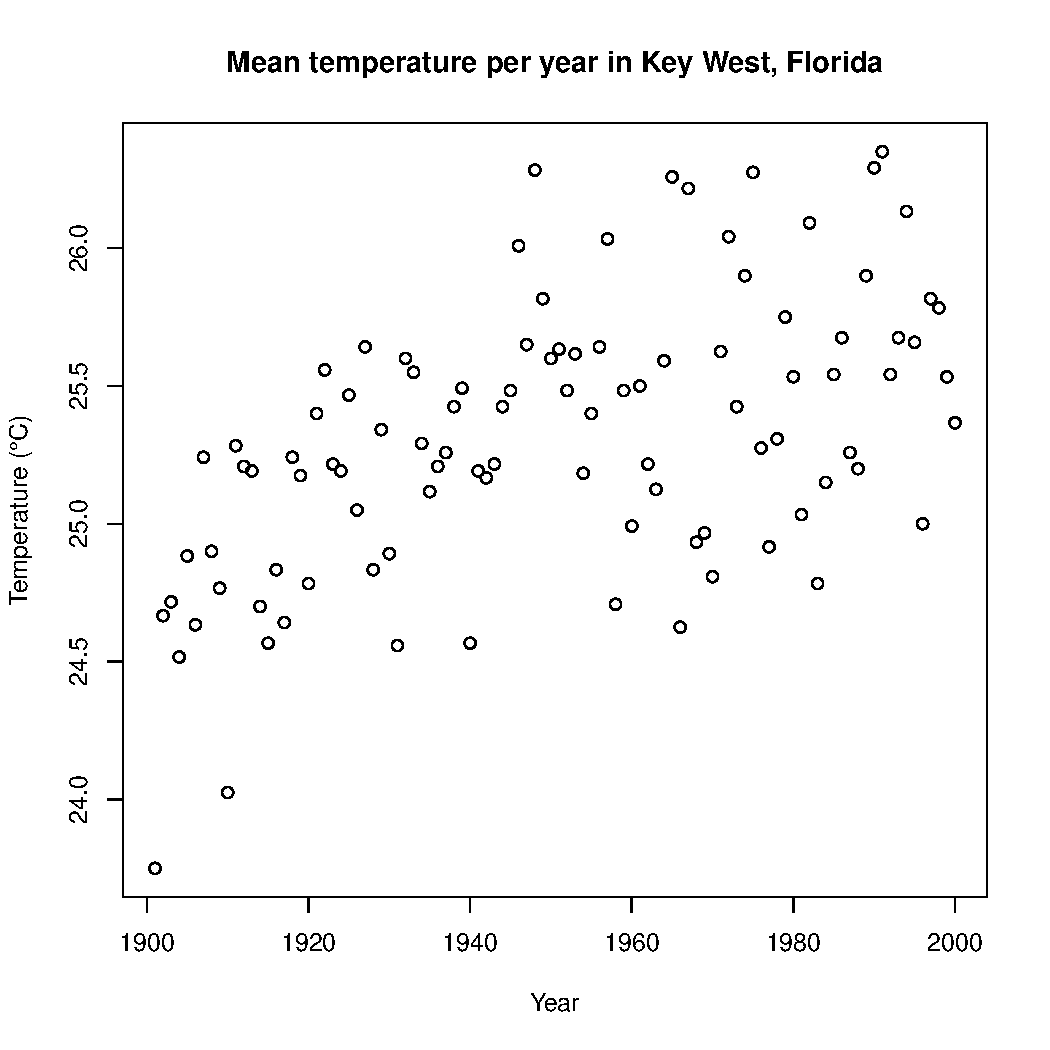
\includegraphics[width=\linewidth]{TAutoPlot1.pdf}
	\caption{Mean temp per year 1900-2000} 
\end{figure}

Figure 1 shows the increase in mean yearly temperature at the study site, from 1900 to 2000. After running the above source code we calculated a p-value $<$ 0.05. This indicates a statistically significant result, therefore we reject the null hypothesis that there is no correlation between lag-1 year mean temperatures. 

\section{Discussion}
The results indicate a significant correlation between temperatures of successive years in Key West, Florida. These findings support previous studies that show spacial and temporal autocorrelation of temperature is present in historical data  \cite{di2018increased}\cite{koenig2016temporally}. Understanding spacial and temporal variation in temperatures is essential in predicting the effects of climate change on ecological communities. Previous studies have shown an increase in autocorrelated temperature through the later half of the 20th Century \cite{dillon2016life}. If this trend continues there may be increased environmental homogenization globally \cite{wu2012enhanced}.

\section{Conclusion}
Our investigation found autocorrelation of temperatures in Key West, Florida. This supports previous studies that have found increasing correlation of temperatures across successive years. This homogenization of global temperatures risks destabilising both terrestrial and marine ecological communities. Serious action to cut carbon emissions must be taken to mitigate the harmful impact of temperature rise on biodiversity.

\bibliographystyle{plain}
\bibliography{TAutoCorrBib}


\end{document}


